\documentclass{standalone}
\usepackage{tikz}
\usetikzlibrary{patterns, positioning}


\begin{document}
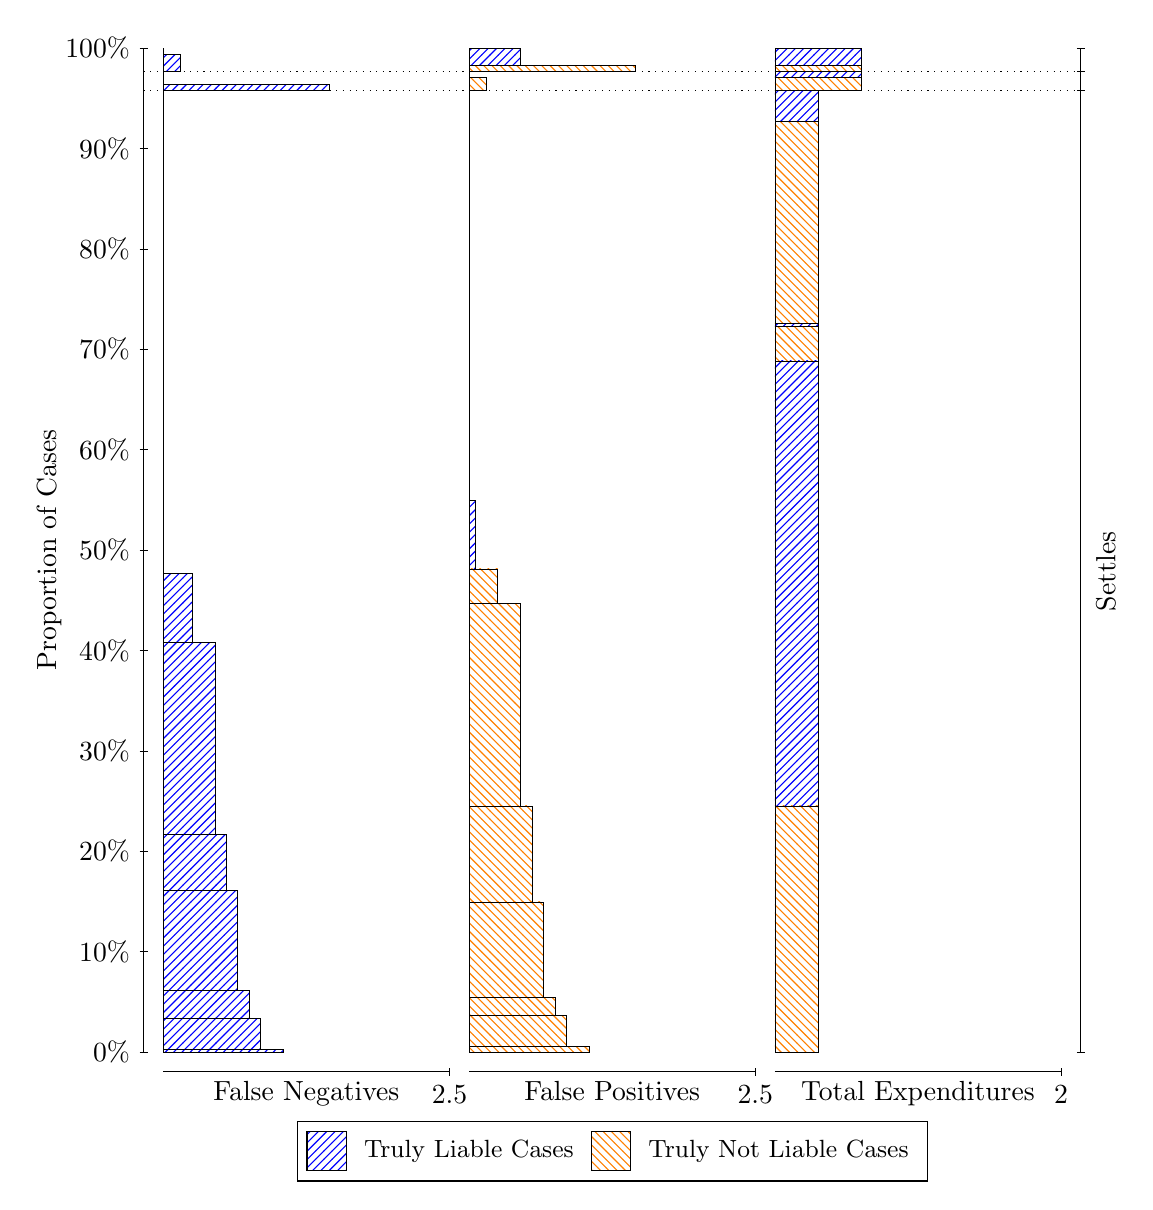
\begin{tikzpicture}
\draw[black, very thin] (1.5,1.75) -- (1.5,14.5);
\node[rotate=90, text=black, anchor=center] at (0.3, 8.125) {Proportion of Cases};
\draw[black, very thin] (1.45,1.75) -- (1.55,1.75);
\node[text=black, anchor=east] at (1.45, 1.75) {0\%};
\draw[black, very thin] (1.45,3.025) -- (1.55,3.025);
\node[text=black, anchor=east] at (1.45, 3.025) {10\%};
\draw[black, very thin] (1.45,4.3) -- (1.55,4.3);
\node[text=black, anchor=east] at (1.45, 4.3) {20\%};
\draw[black, very thin] (1.45,5.575) -- (1.55,5.575);
\node[text=black, anchor=east] at (1.45, 5.575) {30\%};
\draw[black, very thin] (1.45,6.85) -- (1.55,6.85);
\node[text=black, anchor=east] at (1.45, 6.85) {40\%};
\draw[black, very thin] (1.45,8.125) -- (1.55,8.125);
\node[text=black, anchor=east] at (1.45, 8.125) {50\%};
\draw[black, very thin] (1.45,9.4) -- (1.55,9.4);
\node[text=black, anchor=east] at (1.45, 9.4) {60\%};
\draw[black, very thin] (1.45,10.675) -- (1.55,10.675);
\node[text=black, anchor=east] at (1.45, 10.675) {70\%};
\draw[black, very thin] (1.45,11.95) -- (1.55,11.95);
\node[text=black, anchor=east] at (1.45, 11.95) {80\%};
\draw[black, very thin] (1.45,13.225) -- (1.55,13.225);
\node[text=black, anchor=east] at (1.45, 13.225) {90\%};
\draw[black, very thin] (1.45,14.5) -- (1.55,14.5);
\node[text=black, anchor=east] at (1.45, 14.5) {100\%};

\draw[black, very thin] (13.4,1.75) -- (13.4,14.5);
\draw[black, very thin] (13.35,1.75) -- (13.45,1.75);
\node[anchor=west] at (13.35, 1.75) {};
\draw[black, very thin] (13.35,13.959) -- (13.45,13.959);
\node[anchor=west] at (13.35, 13.959) {};
\draw[black, very thin] (13.35,14.2) -- (13.45,14.2);
\node[anchor=west] at (13.35, 14.2) {};
\draw[black, very thin] (13.35,14.5) -- (13.45,14.5);
\node[anchor=west] at (13.35, 14.5) {};

\draw[black, very thin, pattern color=blue, pattern=north east lines] (1.75,1.75) rectangle (3.276,1.7875);
\draw[black, very thin, pattern color=blue, pattern=north east lines] (1.75,1.7875) rectangle (2.9853,2.1736);
\draw[black, very thin, pattern color=blue, pattern=north east lines] (1.75,2.1736) rectangle (2.84,2.5332);
\draw[black, very thin, pattern color=blue, pattern=north east lines] (1.75,2.5332) rectangle (2.6947,3.799);
\draw[black, very thin, pattern color=blue, pattern=north east lines] (1.75,3.799) rectangle (2.5493,4.5137);
\draw[black, very thin, pattern color=blue, pattern=north east lines] (1.75,4.5137) rectangle (2.404,6.9482);
\draw[black, very thin, pattern color=blue, pattern=north east lines] (1.75,6.9482) rectangle (2.1133,7.8254);
\draw[black, very thin, pattern color=orange, pattern=north west lines] (1.75,7.8254) rectangle (1.75,13.959);
\draw[black, very thin, pattern color=blue, pattern=north east lines] (1.75,13.959) rectangle (3.8573,14.036);
\draw[black, very thin, pattern color=orange, pattern=north west lines] (1.75,14.036) rectangle (1.75,14.2);
\draw[black, very thin, pattern color=blue, pattern=north east lines] (1.75,14.2) rectangle (1.968,14.423);
\draw[black, very thin, pattern color=orange, pattern=north west lines] (1.75,14.423) rectangle (1.75,14.5);
\draw[black, very thin, pattern color=orange, pattern=north west lines] (5.6333,1.75) rectangle (7.1593,1.825);
\draw[black, very thin, pattern color=orange, pattern=north west lines] (5.6333,1.825) rectangle (6.8687,2.2178);
\draw[black, very thin, pattern color=orange, pattern=north west lines] (5.6333,2.2178) rectangle (6.7233,2.445);
\draw[black, very thin, pattern color=orange, pattern=north west lines] (5.6333,2.445) rectangle (6.578,3.6552);
\draw[black, very thin, pattern color=orange, pattern=north west lines] (5.6333,3.6552) rectangle (6.4327,4.8756);
\draw[black, very thin, pattern color=orange, pattern=north west lines] (5.6333,4.8756) rectangle (6.2873,7.4453);
\draw[black, very thin, pattern color=orange, pattern=north west lines] (5.6333,7.4453) rectangle (5.9967,7.8839);
\draw[black, very thin, pattern color=blue, pattern=north east lines] (5.6333,7.8839) rectangle (5.706,8.761);
\draw[black, very thin, pattern color=blue, pattern=north east lines] (5.6333,8.761) rectangle (5.6333,13.959);
\draw[black, very thin, pattern color=orange, pattern=north west lines] (5.6333,13.959) rectangle (5.8513,14.123);
\draw[black, very thin, pattern color=blue, pattern=north east lines] (5.6333,14.123) rectangle (5.6333,14.2);
\draw[black, very thin, pattern color=orange, pattern=north west lines] (5.6333,14.2) rectangle (7.7407,14.277);
\draw[black, very thin, pattern color=blue, pattern=north east lines] (5.6333,14.277) rectangle (6.2873,14.5);
\draw[black, very thin, pattern color=orange, pattern=north west lines] (9.5167,1.75) rectangle (10.062,4.8756);
\draw[black, very thin, pattern color=blue, pattern=north east lines] (9.5167,4.8756) rectangle (10.062,10.527);
\draw[black, very thin, pattern color=orange, pattern=north west lines] (9.5167,10.527) rectangle (10.062,10.966);
\draw[black, very thin, pattern color=blue, pattern=north east lines] (9.5167,10.966) rectangle (10.062,11.003);
\draw[black, very thin, pattern color=orange, pattern=north west lines] (9.5167,11.003) rectangle (10.062,13.573);
\draw[black, very thin, pattern color=blue, pattern=north east lines] (9.5167,13.573) rectangle (10.062,13.959);
\draw[black, very thin, pattern color=orange, pattern=north west lines] (9.5167,13.959) rectangle (10.607,14.123);
\draw[black, very thin, pattern color=blue, pattern=north east lines] (9.5167,14.123) rectangle (10.607,14.2);
\draw[black, very thin, pattern color=orange, pattern=north west lines] (9.5167,14.2) rectangle (10.607,14.277);
\draw[black, very thin, pattern color=blue, pattern=north east lines] (9.5167,14.277) rectangle (10.607,14.5);
\draw[black, dotted] (1.5,13.959) -- (13.4,13.959);
\draw[black, dotted] (1.5,14.2) -- (13.4,14.2);
\draw[black, very thin] (1.75,1.5) -- (5.3833,1.5);
\node[text=black, anchor=north] at (3.5667, 1.5) {False Negatives};
\draw[black, very thin] (5.3833,1.45) -- (5.3833,1.55);
\node[text=black, anchor=north] at (5.3833, 1.45) {2.5};

\draw[black, very thin] (5.6333,1.5) -- (9.2667,1.5);
\node[text=black, anchor=north] at (7.45, 1.5) {False Positives};
\draw[black, very thin] (9.2667,1.45) -- (9.2667,1.55);
\node[text=black, anchor=north] at (9.2667, 1.45) {2.5};

\draw[black, very thin] (9.5167,1.5) -- (13.15,1.5);
\node[text=black, anchor=north] at (11.333, 1.5) {Total Expenditures};
\draw[black, very thin] (13.15,1.45) -- (13.15,1.55);
\node[text=black, anchor=north] at (13.15, 1.45) {2};

\node[text=black, centered, rotate=90] at (13.72, 7.8546) {Settles};



\draw (7.449999999999999,1.5) node[draw=none] (baseCoordinate) {};
\begin{scope}[align=center]
        \matrix[scale=0.5, draw=black, below=0.5cm of baseCoordinate, nodes={draw}, column sep=0.1cm]{
            \node[rectangle, draw, minimum width=0.5cm, minimum height=0.5cm, pattern color=blue, pattern=north east lines] {}; &
            \node[draw=none, font=\small, text=black] (B) {Truly Liable Cases}; &
            \node[rectangle, draw, minimum width=0.5cm, minimum height=0.5cm, pattern color=orange, pattern=north west lines] {}; &
            \node[draw=none, font=\small, text=black] (B) {Truly Not Liable Cases}; \\
            };
\end{scope}

\end{tikzpicture}
\end{document}